\RequirePackage{lineno}
\documentclass{cmspaper}

\def\be{\begin{equation}}
\def\ee{\end{equation}}
\def\met{\not\!\!\vec{E}_{T}}

\usepackage[pdftex]{graphicx}
\usepackage{subfigure}
\usepackage{url}
\usepackage{setspace}
\usepackage{color}


\usepackage{amsmath}
\usepackage[amssymb,thinspace]{SIunits}


% own commands
%=====================
\newcommand{\pT}{\ensuremath{p_\perp}}
\newcommand{\Et}{\ensuremath{E_\perp}}
\newcommand{\dpt}{\ensuremath{\delta \pT/\pT}}
\newcommand{\dE}{\ensuremath{\delta E/E}}
\newcommand{\TeV}{\tera\electronvolt}
\newcommand{\GeV}{\giga\electronvolt}
\newcommand{\MeV}{\mega\electronvolt}
\newcommand{\cm}{\centi\meter}
\newcommand{\mm}{\milli\meter}
\newcommand{\mum}{\micro\meter}
\newcommand{\nm}{\nano\meter}
\newcommand{\kg}{\kilo\gram}
%\newcommand{\ns}{\nano\second}
\newcommand{\pb}{\pico\barn}
\newcommand{\pbi}{\ensuremath{\pb^{-1}}}
\newcommand{\nb}{\nano\barn}
\newcommand{\nbi}{\ensuremath{\nb^{-1}}}
\newcommand{\MET}{\ensuremath{\displaystyle{\not} E_T~}}
\newcommand{\HT}{\ensuremath{H_T~}}
\newcommand{\TODO}{{\bf TODO}}


\begin{document}

%\doublespacing
%\setpagewiselinenumbers
%\modulolinenumbers[5]
\linenumbers


%==============================================================================
% title page for few authors

\begin{titlepage}

% select one of the following and type in the proper number:
   \cmsnote{20010/???}
%  \internalnote{2005/000}
%  \conferencereport{2005/000}
   \date{27 October 2010}

  \title{Opposite sign di-lepton SUSY search at $\sqrt{s}=7$~TeV}

  \begin{Authlist}
      M.~Edelhoff, L.~Feld, N.~Mohr, D.~Sprenger
       \Instfoot{iphysb}{I. Physikalisches Institut B, RWTH Aachen University, Germany}
  \end{Authlist}

  \begin{abstract}
  We present a search for Supersymmetry in opposite sign di-lepton final states 
  using the data from 2010 proton-proton-running of the Large Hadron Collider. 
  %The full event selection is based purely on the particle flow event reconstruction.
  The final state signature consists of leptons, several hard jets 
  and missing transverse energy. 
  Since we observe good agreement of data to simulation and our background prediction methods,
  we conclude that there is no sign of flavour correlated di-lepton production 
  accompanied by high jet activity and large missing transverse energy in the dataset of 34~\pbi.
  We report an upper limit on the flavour correlated production of a new physics model within
  acceptance of our event selection.
  \end{abstract} 

\note{Preliminary version}
  
\end{titlepage}

\setcounter{page}{2}%JPP

\tableofcontents 

\graphicspath{{plots/}}

% main part
%============
\section{Disclaimer}

Please note that most of the methods used in this analysis have also been documented in SUS-08-004,
SUS-09-002 (AN-2009/83) and AN-2010/167.

\section{Introduction}

The standard model of particle physics (SM) leads to a number of unsolved issues like the 
hierarchy problem and it provides no solution for pressing questions arising from astrophysical 
observations, most notably dark matter. In Supersymmetry (SUSY) a natural candidate for dark matter 
can be found if R-parity conservation is assumed. Supersymmetric particles (sparticles) have not 
been observed up to now which implies that they have to be heavy. 
On the other hand to provide a solution to the hierarchy problem their masses have to be in the TeV range.
These prejudices lead to a signature of (many) hard jets and large missing transverse energy.

The long anticipated and succesfull start of the Large Hadron Collider (LHC) with a center of mass energy of 7~TeV 
allows us to explore this new TeV range very early on. 
Of special interest are robust signatures in leptonic final states which can be probed with the CMS experiment.
If R-parity is conserved the lightest neutralino escapes detection and no mass peaks can be observed 
in SUSY decay chains. 
%A key point after discovery will be the determination of the sparticle properties. 

The purpose of this analysis is to observe or exclude a significant excess of di-leptons 
over the various backgrounds.
The dataset consists of 34~\pbi of proton-proton collisions collected by CMS during LHC
running in 2010.

In Sec.~\ref{sec:signal} we define the signal benchmark points, that are used in this analysis.
Section~\ref{sec:physobj} describes the technical details of the object selection
and in Sec.~\ref{sec:eff} we discuss the measured lepton efficiencies.
Section~\ref{sec:fakes} describes the method used to determine the contribution
of non-prompt leptons in the final event selection.
In Sec.~\label{sec:eventselection} we define the signal region, which includes a discussion of the main
expected standard model backgrounds and their yields. Here we also discuss the trigger and its efficiency.
Section~\ref{sec:ofossubtraction} deals with the background prediction method (opposite flavour subtraction),
which is used to predict the number of top-pair events in the signal region. We also define a control
region in data and test that the method holds.
The results are presented in Sec.~\ref{sec:results} and we discuss the main sources of systematic
uncertaintes in Sec.~\ref{sec:systematics}. Finally we set a limit and conclude.

\section{Signal}\label{sec:signal}

The CMS minimal supergravity low-mass benchmark points
have been designed to cover 
different decay modes of the neutralinos within supersymmetry. 
The mass spectra of the benchmark points have been calculated using the Softsusy code~\cite{softsusy}. 
All branching ratios have been calculated with the SUSYHit program~\cite{susyhit} 
and the events are simulated using Pythia~\cite{pythia}. 
The k-factor for the cross section at 7~TeV is calculated using a modified version of Prospino~2~\cite{prospino}. 
In mSUGRA observable signal is produced strongly followed be (very) long decay chains 
leading to several hard jets (at least two). 
The escaping neutralino leads to missing transverse energy. 
This fact allows to define a search region to observe an excess over the SM 
and is used as main event selection as described in Section~\ref{sec:eventselection}.

Our signal region are defined as follows
\begin{itemize}
\item Two isolated opposite sign same flavour leptons within acceptance of $p_{T,1}>20$~GeV and $p_{T,2}>10$~GeV.
\item The preselection region requires in addtion $\HT > 100$~GeV, $\MET>100$~GeV
\item The 2010 signal region $\HT > 350$~GeV, $\MET>150$~GeV
\item We define a high \HT signal region $\HT > 600$~GeV, $\MET>100$~GeV
\item We define a high \MET signal region $\HT > 250$~GeV, $\MET>250$~GeV
\end{itemize}

This definition is based on our prejudice of heavy objects
being pair produced decaying subsequently through a cascade
including an opposite sign lepton pair.

%\begin{figure}[hbtp]
%\begin{center}
%\subfigure[]{\label{fig:yieldOSByChannelAndBMPoint}\includegraphics[angle=0,width=0.49\textwidth]{diLepton342_combinedOSpromptPromptTauCount}}\hfill
%\end{center}
%     \subfigure[]{\label{fig:yieldSSByChannelAndBMPoint}\includegraphics[angle=0,width=0.49\textwidth]{diLepton342_combinedSSpromptPromptTauCount}}\hfill
% \caption{Expected event yield for a given benchmark point and exclusive di-lepton channel with respect to the total expected di-lepton
%    event yield at that benchmark point. Only the hadronic decay of the $\tau$-lepton is counted in the ``Tau'' channels, as
%    this is the distinction that is made on detector level.\label{fig:yieldByChannelAndBMPoint}}
%\end{figure}

%The number of expected events in a given di-lepton channel varies with the mSUGRA point realised by nature. 
%Thus, itsimportance cannot be judged from a single point in mSUGRA phase-space. 
%A range of benchmark points has been studied to anticipate different possible signal constellations and not
%tune towards a specific set of parameters. 
%Figure~\ref{fig:yieldByChannelAndBMPoint} shows the fraction of di-leptonic events splitted by flavour
%for a di-lepton selection on generator level. In all studied benchmark points
%the flavour correlated production dominates over the uncorrelated production.



\section{Physics objects}\label{sec:physobj}

\subsection{PAT workflow}

From the AOD samples so called Pat-Tuples have been created using the following 
tags of the Physics Analysis Toolkit (PAT) in CMSSW\_4\_2\_X. 
\begin{verbatim}
cmsrel CMSSW_4_2_3
cd CMSSW_4_2_3/src
cmsenv
addpkg PhysicsTools/PatAlgos    V08-06-25
addpkg PhysicsTools/PatExamples V00-05-17

# deterministic calculation of FastJet corrections
addpkg RecoJets/Configuration                           V02-04-16
addpkg RecoJets/JetAlgorithms                           V04-01-00      
addpkg RecoJets/JetProducers                            V05-05-03

addpkg MuonAnalysis/MuonAssociators                  V01-13-00
addpkg PhysicsTools/Configuration                         V00-10-14

addpkg RecoTauTag/RecoTau RecoTauDAVerticesPatch_V5  
addpkg RecoTauTag/TauTagTools RecoTauDAVerticesPatch_V5
addpkg RecoTauTag/Configuration RecoTauDAVerticesPatch_V5

cvs co -d__temp__ -r1.1 UserCode/SuSyAachen/Configuration/python/pfTools.py
/bin/mv __temp__/pfTools.py PhysicsTools/PatAlgos/python/tools
rm -r __temp__


cvs co -rV00-04-48 -dSuSyAachen UserCode/SuSyAachen
\end{verbatim}

All physics objects necessary for this analysis are included in the Pat-Tuples.

\subsection{Datasets}

We perform the analysis on events triggered by leptonic, hadronic
and cross-object triggers
and therefore use several primary datasets
reconstructed in CMSSW\_4\_2\_X.
All datasets used are listed in Tab.~\ref{tab:datadatasets}.
\begin{table}[htdp]
\caption{Datasets used in this analysis.}
\label{tab:datadatasets}
\begin{center}
\begin{tabular}{|l|} \hline
    DBS datasetpath    \\ \hline \hline % &   No. events    & Luminosity [pb$^{-1}$]   \\ \hline \hline
/DoubleElectron/Run2011A-May10ReReco-v1/AOD \\ 
/DoubleElectron/Run2011A-PromptReco-v4/AOD\\
/DoubleMu/Run2011A-May10ReReco-v1/AOD\\ 
/DoubleMu/Run2011A-PromptReco-v4/AOD\\
/MuEG/Run2011A-May10ReReco-v1/AOD\\ 
/MuEG/Run2011A-PromptReco-v4/AOD\\\hline
/ElectronHad/Run2011A-May10ReReco-v1/AOD \\ 
/ElectronHad/Run2011A-PromptReco-v4/AOD \\ 
/MuHad/Run2011A-May10ReReco-v1/AOD \\
/MuHad/Run2011A-PromptReco-v4/AOD\\\hline 
/HT/Run2011A-May10ReReco-v1/AOD \\ 
/HT/Run2011A-PromptReco-v4/AOD \\ \hline 
\end{tabular}
\end{center}
\end{table}

We select only events that enter the officially produced good-run-list
\begin{verbatim}
/afs/cern.ch/cms/CAF/CMSCOMM/COMM_DQM/certification/Collisions11/7TeV/Reprocessing/
Cert_160404-163869_7TeV_May10ReReco_Collisions11_JSON.txt
\end{verbatim}
and the total integrated luminosity amounts to
\begin{equation}
\mathcal{L}_{int} = (204\pm8)~\pbi.
\end{equation}

\subsection{Simulated datasets}

All simulated samples from CMSSW\_4\_2\_X are listed in Tab~\ref{tab:alldataset}. 
Please note that for the
final version the proper Madgraph samples will be used (as soon as they are 
available).
 
\begin{table}[htdp]
\caption{Used CMSSW datasets from 4\_2\_X.}
\label{tab:alldataset}
\begin{center}
%\begin{small}
\begin{tabular}{|l||c||c||c|} \hline
 	DBS datasetpath 	&	No. events 		&   $\sigma_{LO}$ [pb] & Name\\ \hline \hline
/LMX\_SUSY\_sftsht\_7TeV-pythia6/Fall10-START38\_V12-v1/AODSIM & 200000 & varies & SUSY LMX\\ \hline
/TTJets\_TuneZ2\_7TeV-madgraph-tauola/Fall10-START38\_V12-v2/AODSIM& 1443404 & 90& tt+jets\\ \hline
/DYJetsToLL\_TuneZ2\_M-50\_7TeV-madgraph-tauola/Fall10-START38\_V12-v2/AODSIM & 1084921 & 2350& Z+jets\\ \hline
/WToENu\_TuneZ2\_7TeV-pythia6/Fall10-START38\_V12-v1/AODSIM & 189069 & 8057& W+jets\\ \hline
/WToMuNu\_TuneZ2\_7TeV-pythia6/Fall10-START38\_V12-v1/AODSIM & 189069 & 8057& W+jets\\ \hline
/WToTauNu\_TuneZ2\_7TeV-pythia6/Fall10-START38\_V12-v1/AODSIM & 189069 & 8057& W+jets\\ \hline
/QCD\_TuneD6T\_HT-100To250\_7TeV-madgraph/Fall10-START38\_V12-v1/AODSIM & 10842371 & 7000000 & QCD\\ \hline
/QCD\_TuneD6T\_HT-250To500\_7TeV-madgraph/Fall10-START38\_V12-v1/AODSIM & 4873036 & 171000 & QCD\\ \hline
/QCD\_TuneD6T\_HT-500To1000\_7TeV-madgraph/Fall10-START38\_V12-v1/AODSIM & 4034762 & 520& QCD\\ \hline
/QCD\_TuneD6T\_HT-1000ToInf\_7TeV-madgraph/Fall10-START38\_V12-v1/AODSIM & 1541261 & 83 & QCD\\ \hline
%\multicolumn{3}{|l|}{$^{\dagger}$GEN-SIM-DIGI-RECO} \\ \hline
\end{tabular}
%\end{small}
\end{center}
\end{table}

Each dataset is scaled to the desired luminosity if not illustrated differently. 
Additionally a k-factor has been applied for some of the datasets.
The MC is reweighted to correct for the difference in the vertex
multiplicity distribution as described in \cite{pileup}.

\subsection{Common event selection}\label{sec:cleanup}
To select good collision events we require the event to contain a good primary vertex,
which has to pass the following conditions
\begin{verbatim}
!isFake
ndof > 4
abs(z) <= 24
position.Rho <= 2.
\end{verbatim}

\subsection{Muons}\label{sec:muons}

 The acceptance of the muons is restricted to $p_T>5$~GeV %(Fig.~\ref{fig:muon_pt}) 
and $|\eta|<2.4$. 
Each muon has to be identified as a global muon and tracker muon. 
The track of the muon in the inner tracker has to have at least 11 hits
and a $\chi^2/ndf$ of the global muon track below 10. 
The impact parameter of the muon track with respect to the position of the first 
deterministic annealing (DA) vertex is 
required to be below $200$~$\mu$m in $x$-$y$ and within $1$~cm in $z$.
Additionally we require the muons to be well measured by the request that the
relative error from the track-fit is below 10\%. 
The combined energy sum in cone of size dR = 0.3 around each muon has
to be smaler than 15\% of its energy.
All cuts are summarised in Table~\ref{tab:Muons}.

    \begin{table}[hbtp]
    \caption{Overview of the muon selection.\label{tab:Muons}}
    \vspace{0.4cm}
    \begin{center}
    \begin{tabular}{|c||c||c|} \hline
Name&Pat memberfunction & Cut\\\hline \hline
p$_{T}$ & pt() & $\ge 5.$ \\\hline 
$|\eta|$ & abs(eta()) & $\le 2.4$ \\\hline 
GlobalPromptTight& muonID( 'GlobalMuonPromptTight' ) & \\\hline 
TrackerMuon& isTrackerMuon() & \\\hline 
Number of hits& track.numberOfValidHits  & $\ge 11$\\\hline 
%Number of pixel hits& track.numberOfValidPixelHits  & $\ge 1$\\\hline 
Good track fit& track.ptError()/track.pt()  & $\leq 0.1$\\\hline 
Impact parameter& abs(dxy(pv))  & $ \le 0.02$\\\hline 
Impact parameter& abs(dz(pv))  & $ \le 1$\\\hline 
Isolation& (isolationR03().hadEt + isolationR03().emEt + isolationR03().sumPt) / pt  & $\le 0.15$\\\hline 
\end{tabular}
    \end{center}
    \end{table}


\subsection{Electrons}\label{sec:electrons}

%The electron collection~\cite{electrons} is derived from the particle flow electron collection and provided by PF2PAT. 
The acceptance of the electrons is restricted to $p_T>10$~GeV %(Fig.~\ref{fig:electron_pt}) 
and $|\eta|<2.5$. 
We restrict ourselves to the ECALs fiducial volume,
thus exclude electrons within $1.4442 < \eta < 1.566$.

%(Fig.~\ref{fig:electron_eta}) 
Additionally, a conversion rejection
is performed requiring that the electron track has maximally one lost hit in the tracker.
We remove electrons from conversions via partner track finding, i.e. if there is a general track within
$Dist < 0.02$~cm and $\Delta \cot \theta < 0.02$ \cite{conv}.
The impact parameter of the electron track with respect to the position 
of the primary DA vertex position is required to be 
below $400$~$\mu$m in $x$-$y$ and smaller than $1$~cm in $z$.
The cuts are summarised in Table~\ref{tab:Electrons}.

    \begin{table}[hbtp]
    \caption{Overview of the electron selection.\label{tab:Electrons}}
    \vspace{0.4cm}
    \begin{center}
    \begin{tabular}{|c||c||c|} \hline
Name&Pat memberfunction & Cut\\\hline \hline
p$_{T}$ & pt() & $\ge 5.$ \\
$|\eta|$ & abs(eta()) & $\le 2.4$ \\\hline 
Identification & WP95 &  \\\hline 
%Energy over momentum& eSuperClusterOverP & $\le$ 1.7 \\\hline 
Lost hits& gsfTrack--\textgreater trackerExpectedHitsInner().numberOfHits()  & $\le 1$\\
Partner track finding&  !($|Dist|  and |\Delta \cot \theta|$ )  & < 0.02\\\hline 
Impact parameter& abs(dxy(pv))  & $ \le 0.04$\\ 
Impact parameter& abs(dz(pv))  & $ \le 1$\\\hline 
Isolation Barrel& (dr03HcalTowerSumEt + max( 0., dr03EcalRecHitSumEt-1. ) + dr03TkSumPt) / pt & $\le 0.15$\\
Isolation Barrel& (dr03HcalTowerSumEt + dr03EcalRecHitSumEt + dr03TkSumPt) / pt & $\le 0.15$\\\hline 
\end{tabular}
    \end{center}
    \end{table}

\subsection{Light lepton isolation}\label{sec:isolation}

A combined relative lepton isolation has been used. The isolation uses information from both calorimeters and the silicon tracker. The isolation value ($Iso$) is given by the ratio of the sum of all $p_T$ objects within a cone in $\eta$-$\phi$-space of $\Delta R = \sqrt{\Delta \eta^2 + \Delta \phi^2 } < 0.4$ around the lepton and the lepton $p_T$. It has been pre-calculated in PAT using
\be
    Iso = \frac{ \displaystyle \left[ \sum_{photons}{p_{T}}+\sum_{neutral \; hadrons}{p_{T}}+\sum_{charged \; hadrons} {p_{T}}\right]_{dR<0.4}}{p_T}
\ee
where the first sum runs over the transverse momentum of all particle flow photons, the second sum runs over the transverse momentum of all neutral hadrons and the third sum runs over the transverse momentum deposited as charged hadrons within the cone.


The isolation for prompt muons obtained from the sPlot technique (Sec.\ref{sec:splot}) is shown Figure~\ref{fig:muon_iso} and the cut value is chosen to be $Iso<0.2$. The distribution for electrons is displayed in Figure~\ref{fig:electron_iso} and the cut is placed at $Iso<0.2$ to obtain a similar rejection and efficiency for electrons and muons. The background shapes evaluated from data are discussed in Sec.~\ref{sec:fakes}.

\subsection{Taus}\label{sec:taus}

\TODO: Matthias tau selection

\subsection{Jets and missing transverse energy}\label{sec:jet}

The anti-kt jet algorithm~\cite{antiKT} with a cone size of 0.5 in $\Delta R$ is used. 
Jets are clustered from all reconstructed particle flow particles.
We remove jets that are within $\Delta R < 0.4$ to a lepton passing our
full lepton selection. Thus we obtain fully lepton cleaned jets in our final selection.
The jets are corrected up to level 3 using MC jet energy corrections~\cite{mcjetcorrections}
from the Summer11 (GlobalTag: GR\_R\_42\_V12, START42\_V12) production. 
To correct for PileUp the L1FastJet subtraction using the latest JetMET
prescription is applied.

Each corrected jet is required to have a $p_T$ above 30 GeV and 
the jet axis has to be within $|\eta| < 3$. This relatively tight $\eta$ cut is used 
to be able to include tracker information in the jet identification for a large part of the $\eta$ acceptance and 
not to rely on the hadronic calorimeter only. 
Thus, one is able to fully profit from the particle flow algorithm.
Each jet has to pass the "FIRSTDATA" "LOOSE" Particle Flow Jet ID criteria, which
are used to suppress fake, noise, and badly reconstructed jets, while
still retaining as much real jets as possible~\cite{pfjetid}.

The missing transverse energy (MET) is based on the sum of all particle 
momenta reconstructed using the particle flow event reconstruction (pfMET).

\subsection{Trigger}\label{sec:trigger}

We collect events using three different trigger streams:
\begin{itemize}
\item (20,10) GeV $ee$, $e\mu$, $\mu\mu$ events are selected using the lepton trigger selection.
\item (10,10), (10,5), (5,5) GeV $ee$, $e\mu$, $\mu\mu$ events are selected using the lepton \HT cross object trigger selection.
\item (5,15), (10,15), (15,15) GeV $\mu\tau$, $e\tau$, $\tau\tau$ events are selected using the tau trigger selection.
\end{itemize}

\subsubsection{Lepton trigger selection}
To collect events for the (20,10) GeV di-lepton selection
we use an OR of the following double lepton high level trigger (HLT) paths
\begin{itemize}
\item HLT\_Ele17\_CaloIdL\_CaloIsoVL\_Ele8\_CaloIdL\_CaloIsoVL\_v* 
\item HLT\_Ele17\_CaloIdT\_TrkIdVL\_CaloIsoVL\_TrkIsoVL\_Ele8\_CaloIdT\_TrkIdVL\_CaloIsoVL\_TrkIsoVL\_v* 
\item HLT\_Mu8\_Ele17\_CaloIdL\_v* 
\item HLT\_Mu17\_Ele8\_CaloIdL\_v* 
\item HLT\_Mu10\_Ele10\_CaloIdL\_v* 
\item HLT\_DoubleMu6* 
\item HLT\_DoubleMu7\_v* 
\item HLT\_Mu13\_Mu7\_v*
\end{itemize}
We check that the prescale of each trigger is set to one
for all run ranges.

We measure the eficiency in an orthogonal event selection
using events triggered by purely hadronic triggers.

%\begin{figure}[hbtp]
%  \subfigure[]{\label{fig:htTrigger}\includegraphics[width=0.79\textwidth]{HTTriggerTurnOn.pdf}}\hfill
%  \caption{\HT-trigger turn-on curve with respect to our definition of \HT measured on a muon triggered control sample. The slow turn-on comes from the much better resolution of particle flow jets compared to uncorrected calo jets used in the trigger.}
%\end{figure}

\begin{table}[hbtp]
\caption{Double lepton high level trigger efficiencies. \label{tab:Trigger}}
\begin{center}
\begin{tabular}{|l||c|c|c|} \hline
HLT path    &   Thresh. [GeV]   &   Pathname        & $\epsilon$\\\hline \hline
\HT &   100 & HLT\_HT100U    &$99.8\pm0.1$\% \\\hline  
\HT &   140 & HLT\_HT140U    &$99.7\pm0.1$\% \\\hline  
\HT &   150 & HLT\_HT150U    &$99.7\pm0.1$\% \\\hline  
\end{tabular}
\end{center}
\end{table}

The measured efficiencies are listed in Table~\ref{tab:Trigger}. 
We obtain an efficiency of $(99.7\pm0.1)$\%, ($(99.7\pm0.1)$\%, $(99.7\pm0.1)$\%) 
for the $ee$ ($e\mu$, $\mu\mu$) trigger with respect to the final 
di-lepton selection, respectively.

\subsubsection{Lepton $H_T$ cross trigger trigger selection}
To collect events for low lepton $p_T$ range ($e$ 10, $\mu$ 5) GeV di-lepton plus
$\HT$ cross-object triggers are used.
We use an OR of the following double lepton \HT HLT paths
\begin{itemize}
\item HLT\_DoubleEle8\_CaloIdL\_TrkIdVL\_HT160\_v* 
\item HLT\_DoubleEle8\_CaloIdL\_TrkIdVL\_HT150\_v* 
\item HLT\_DoubleMu3\_HT160\_v* 
\item HLT\_DoubleMu3\_HT150\_v* 
\item HLT\_Mu3\_Ele8\_CaloIdL\_TrkIdVL\_HT160\_v* 
\item HLT\_Mu3\_Ele8\_CaloIdL\_TrkIdVL\_HT150\_v*
\end{itemize}
We check that the prescale of each trigger is set to one
for all run ranges.

We measure the leptonic eficiency in event selection
using events triggered by purely hadronic (\HT) triggers,
while the hadronic efficiency is measured using
events collected by di-lepton triggers. We assume
no correlation between the hadronic and leptonic
part of the trigger and give the total efficiency
as a product of both.

\begin{table}[hbtp]
\caption{Double lepton \HT cross object trigger high level trigger efficiencies. \label{tab:TriggerHT}}
\begin{center}
\begin{tabular}{|l||c|c|c|} \hline
HLT path    &   Thresh. [GeV]   &   Pathname        & $\epsilon$\\\hline \hline
\HT &   100 & HLT\_HT100U    &$99.8\pm0.1$\% \\\hline  
\HT &   140 & HLT\_HT140U    &$99.7\pm0.1$\% \\\hline  
\HT &   150 & HLT\_HT150U    &$99.7\pm0.1$\% \\\hline  
\end{tabular}
\end{center}
\end{table}

The measured efficiencies are listed in Table~\ref{tab:TriggerHT}. 
We obtain an efficiency of $(99.7\pm0.1)$\%, ($(99.7\pm0.1)$\%, $(99.7\pm0.1)$\%) 
for the $ee$ ($e\mu$, $\mu\mu$) trigger with respect to the final 
di-lepton selection, respectively.

\subsubsection{Tau trigger selection}
To collect event including taus in the final state
we use an OR of the following double lepton high level trigger (HLT) paths
\begin{itemize}
\item \TODO tau trigger selection
\end{itemize}
We check that the prescale of each trigger is set to one
for all run ranges.

We measure the eficiency in an orthogonal event selection
using events triggered by purely hadronic triggers.

\begin{table}[hbtp]
\caption{Tau high level trigger efficiencies. \label{tab:TriggerTau}}
\begin{center}
\begin{tabular}{|l||c|c|c|} \hline
HLT path    &   Thresh. [GeV]   &   Pathname        & $\epsilon$\\\hline \hline
\HT &   100 & HLT\_HT100U    &$99.8\pm0.1$\% \\\hline  
\HT &   140 & HLT\_HT140U    &$99.7\pm0.1$\% \\\hline  
\HT &   150 & HLT\_HT150U    &$99.7\pm0.1$\% \\\hline  
\end{tabular}
\end{center}
\end{table}

The measured efficiencies are listed in Table~\ref{tab:TriggerTau}. 
We obtain an efficiency of $(99.7\pm0.1)$\%, ($(99.7\pm0.1)$\%, $(99.7\pm0.1)$\%) 
for the $ee$ ($e\mu$, $\mu\mu$) trigger with respect to the final 
di-lepton selection, respectively.

\section{Efficiency for electrons and muons}\label{sec:eff}

The efficiency ratio is derived directly from the data
but selection of an inclusive Z boson sample.
For this we select di-lepton events ($ee$, $\mu\mu$) 
with (20,10) GeV including the lepton trigger paths
listed in Sec.??.

We apply an cut in the invariant mass of $60 < m_{ll} < 120$~GeV
to obtain a pure Z boson sample. The differnt flavour subtraction 
described in Sec.~\ref{sec:ofossubtraction} relies on the 
knowledge of the electron to muon efficiency ratio, which
we derive from this sample as
\be
    r_{\mu e} = \sqrt{\frac{n_{\mu\mu}}{n_{ee}}} = 1.13 \pm 0.07
\ee

\begin{figure}[hbtp]

  \subfigure[]{\label{fig:cont_iOSee}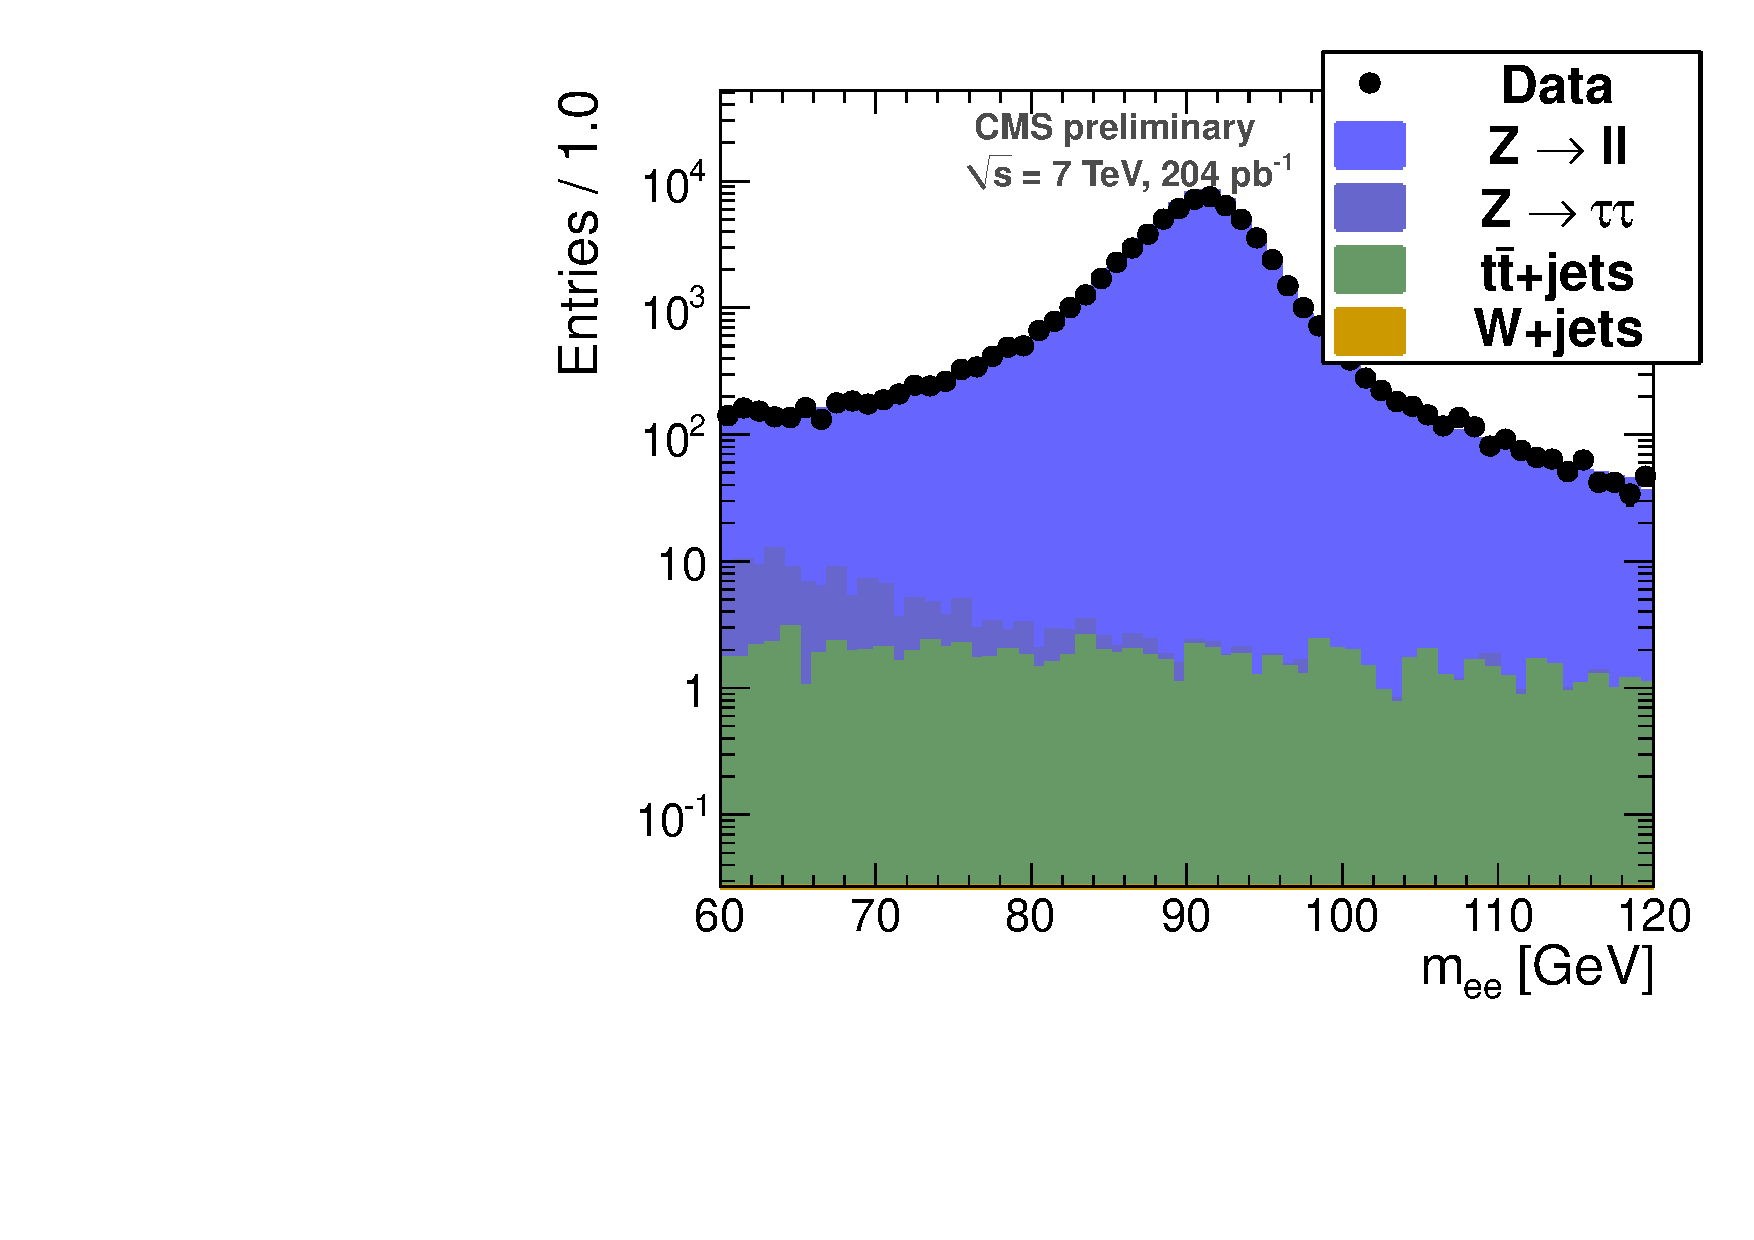
\includegraphics[width=0.49\textwidth]{Summer11_07_MC_pfLeptSusyCuts_Data_iOSee_EE.pdf}}\hfill
  \subfigure[]{\label{fig:cont_iOSmm}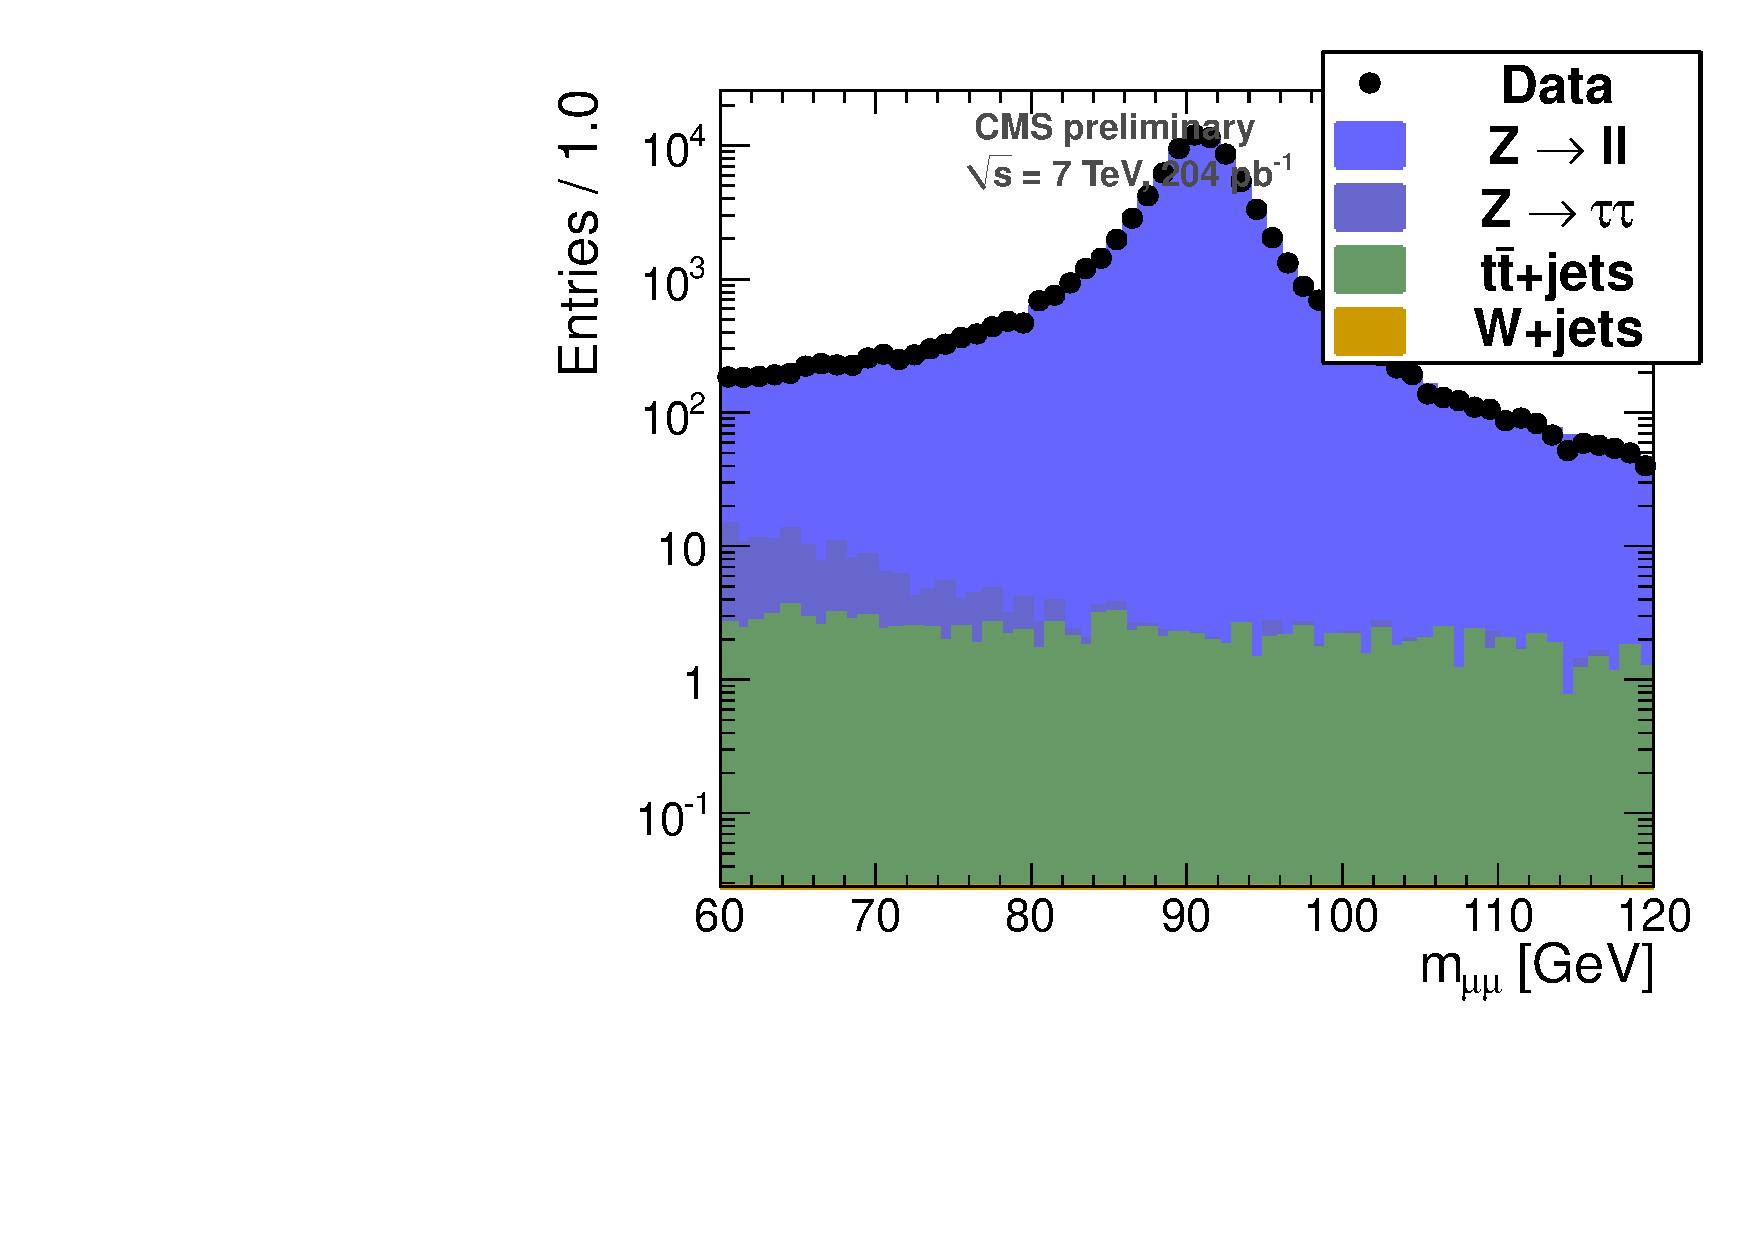
\includegraphics[width=0.49\textwidth]{Summer11_07_MC_pfLeptSusyCuts_Data_iOSmm_MuMu.pdf}}\hfill
  \caption{Invariant mass distributions for a (20,10) GeV di-lepton selection after leptonic 
      trigger requirement.\label{fig:Z_InvMass}}
\end{figure}


\begin{table}[htbp]
\begin{center}
\caption{\label{tab:tnp_eff}Muon to electron reconstruction efficiency ratio 
    obtained from a Z boson selection on data and $Z+\textrm{jets}$ Monte Carlo simulation.} 
\begin{tabular}{lcc}
\hline
            &  Data                                                 & Monte Carlo \\
\hline\hline
\hline
ratio $r_{\mu e}$       & $1.13 \pm 0.005 (\textrm{stat}) \pm 0.07 (\textrm{syst})$    & $1.11 \pm 0.003(\textrm{stat}) $ \\
\hline
\end{tabular}
\end{center}
\end{table}


Since we measure the efficiency on a Z sample, which has a different jet multiplicity
compared to a ttbar sample, we need to assign a systematic uncertainty in the extrapolation.
We test the dependence in simulation by comparing a top MC sample with Z-boson simulation.
While the absolute efficiency drops, the ratio of the electron to muon efficiency
is approximately constant (within $6\%$), meaning that the loss in efficiency is the same for both lepton
flavours. We therefore assume 6\% additional systematic uncertainty on the ratio.

%\section{Fake background measurement}\label{sec:fakes}

The fake lepton background can be measured using an isolation template method~\cite{suspas10001}. From prompt leptons in Z events or from MC, an isolation template for signal leptons can be obtained. We use a data-driven template from the sPlot technique (Sec.~\ref{sec:splot}) to verify, that the isolation is well described by the simulation (Sec.~\ref{sec:physobjects}).
We then use the isolation distribution from simulated prompt leptons in Z boson (includes Drell-Yan) events 
to obtain a signal shape, which are close enough to the isolation distribution in our final signal region.
Using the prompt leptons in this sample, the isolation template is created by fitting a Breit-Wigner convoluted with a gaussian to the isolation distribution (Fig.~\ref{fig:promptMu_fit} shows the signal template for muons and Fig.~\ref{fig:promptEle_fit} displays it for electrons). 

The background component of the lepton isolation distribution, consisting of fake leptons and leptons emerging from decays of heavy quarks, is fitted using a landau function. Figure~\ref{fig:backMu_fit} (muons) and Figure~\ref{fig:backEle_fit} (electron) display the isolation distribution for a di-jet event selection with $\HT > 200$~GeV and $\MET < 20$~GeV. We select only events with one reconstructed lepton to supress the Z contribution. Based on simulation the selection yields a relatively pure QCD sample, while there is still some remaining signal contamintaion for low isolation. The signal contamination leads to a slight overestimation of the fake component. The fitted landau describes the shapes reasonably well. We excluded low isolation region in the fit to test the impact on the prediction and find a shift of 10\%, which is covered by the systematic uncertainty as discussed later.

\begin{figure}[hbtp]
  \subfigure[]{\label{fig:promptMu_fit}\includegraphics[width=0.49\textwidth]{promptFit_muon.pdf}}\hfill
  \subfigure[]{\label{fig:backMu_fit}\includegraphics[width=0.49\textwidth]{backFit_muon.pdf}}\hfill
  \subfigure[]{\label{fig:promptEle_fit}\includegraphics[width=0.49\textwidth]{promptFit_electron.pdf}}\hfill
  \subfigure[]{\label{fig:backEle_fit}\includegraphics[width=0.49\textwidth]{backFit_electron.pdf}}\hfill
  \subfigure[]{\label{fig:fakeLeptElectron}\includegraphics[width=0.49\textwidth]{combinedFit_pfLeptSusyElectron}}\hfill
  \subfigure[]{\label{fig:fakeLeptMuon}\includegraphics[width=0.49\textwidth]{combinedFit_pfLeptSusyMuon}}\hfill
  
  \caption{Fit of the isolation distribution of prompt leptons in a Z simulation sample to create an isolation
    template~\subref{fig:promptMu_fit}. The background muon contribution (di-jet selection on data based on $\HT > 200$~GeV and $\MET < 20$) can be described by a landau
    function~\subref{fig:backMu_fit}. Using the determined isolation template, the number of signal and background leptons in
    the final event selection can be predicted. The fit in the control region (Sec.~\ref{sec:ofossubtraction}) is shown in \subref{fig:fakeLeptElectron} for electrons and \subref{fig:fakeLeptMuon} muons. The measured purity is similar to the expectation from simulation.} %on a $100~\pbi$ MC sample~\subref{fig:combMu_fit}. The dashed curves represent the parts of the fit for the signal (red) and background (green), while the blue line is the combination. The solid histogramms respresent the true contribution of each source in MC.}
\end{figure}

Using this method, the purity of the final lepton selection and hence the fake component in the final event selection can be predicted. 

To measure the purity all analysis cuts (including \HT and \MET selection), except the isolation requirement on both leptons,
are applied. In this sample the purity can be determined by the a simultaneous fit to the signal template, background template and lepton isolation distribution in the final event selection.
Figure~\ref{fig:fakeLeptElectron} shows the fit of the purity for electrons in the control region (Sec.~\ref{sec:ofossubtraction}) and Fig.~\ref{fig:fakeLeptMuon} displays the fit int the same region for the muon sample.
From the impurity ($0.024\pm0.005$ for electrons and $0.013\pm0.002$ for muons) we calculate the predicted 
number of fakes in Sec.~\ref{sec:ofossubtraction}.
The fit in the signal region is shown in Fig.~\ref{fig:fakeHadElectron} for electrons
and Fig.~\ref{fig:fakeHadMuon} displays it for muons.
All additional isolation fits are shown in Appendix~\ref{app:fakefits} as well.

To obtain the fake-yields in the di-electron, di-muon and cross-channel one simply
multiplies the number of candidates in the desired event selection by the impurity.
Here we neglect double-fake events, since in the final signal selection, the expected number of single
fake leptons is already small.

The measured impurity in the final selection and in the control region is found to be smaller than 10-5\%
for the full lepton selection. A closure test on first W Boson data is performed in~\cite{suspas10001}.

We have tested the closure of the method in simulation in the control region 
(fits are shown in Fig.~\ref{fig:fakeMCClosureElectron} and Fig.~\ref{fig:fakeMCClosureMuon}). 
We compare the fake yield with the observed events from 
heavy flavour and fake leptons and find a good closure.
For electrons we predict $5.1\pm0.6$ compared to 4 fakes in MC truth
and for muons we predict $4.8\pm0.4$ compared to 3 fakes in MC truth.

On real data the closure of the method is tested in a W dominated region with
$\MET > 30$~GeV and $\HT>200$~GeV and the fits are shown in
Fig.~\ref{fig:fakeWElectron} and Fig.~\ref{fig:fakeWMuon}.
We observe good agreement of the prompt yield between electron 
and muon channels, but the fake yield differs, because of the
cleaner muon sample.

\subsection{Systematic uncertainty of the method}

The isolation shape is senstive to the lepton $p_T$ distribution which can differ between
between the QCD selection where we derive the template from and the final signal
selection, where we apply the isolation fit.
To assign a systematic uncertainty due to the sampling of the isolation distribution
we test the closure in a background dominated region with $\MET < 20$~GeV and exactly one 
non-isolated lepton passing all identification cuts. Table~\ref{tab:ptVariation} shows the observed
and and predicted number of fakes, when the $p_T$ of the leptons is varied.
We find a variation of up to 40\%, when we vary the lepton $p_T$, which gives the largest
part of the systematic uncertainty of the method.
Table~\ref{tab:htVariation} shows the observed
and and predicted number of fakes, when the \HT of the selction is varied.
The variation with \HT is not as strong as for the lepton $p_T$ and we find a variation of 30\%.

\begin{table}[hbtp]
\caption{Variation of prediction vs. obeservation for lepton candidates with different $p_T$'s in a background dominated region with $\MET < 20$~GeV, $\HT > 200$~GeV and exactly one lepton.\label{tab:ptVariation}}
\begin{center}
\begin{tabular}{|l||c|c|c|c|} \hline
   $p_T$ [GeV]   &   10-15 &  15-20  & 20-25 & 25-60 \\\hline \hline
Electron pred./obs. &   55/68    & 45/32 & 34/24 & 93/80 \\\hline  
Relative change &   -20\%    & +40\% & +41\% & +16\% \\\hline  
Muon pred./obs. &   26/31    & 12/19 & 12/14 & 34/26 \\\hline  
Relative change &   -17\%    & -37\% & +15\% & +36\% \\\hline  
\end{tabular}
\end{center}
\end{table}

\begin{table}[hbtp]
\caption{Variation of of prediction vs. obeservation for lepton candidates with different \HT in a background dominated region with $\MET < 20$ and exactly one lepton.\label{tab:htVariation}}
\begin{center}
\begin{tabular}{|l||c|c|c|c|} \hline
   \HT [GeV]   &  100-120   &  140-160  & 200-300  & $> 300$ \\\hline \hline
Electron &   338/391    & 300/267 & 221/178 & 46/52 \\\hline  
Relative change &   -14\%    & +12\% & +24\% & -12\% \\\hline  
Muon &   116/116    & 80/83 & 150/135 & 28/20 \\\hline  
Relative change &   -    & -4\% & +12\% & +40\% \\\hline  
\end{tabular}
\end{center}
\end{table}


In total we assign a systematic uncertainty of 50\% on the prediction.

%Figure~ shows the fits in the control and signal region on data, which we use
%to derive the fake-prediction in the control region (Sec.~\ref{sec:ofossubtraction}) and 
%signal region Sec.~\ref{sec:results}.

%{\textcolor{red} To give a more comprehensive overview over the fake template method, we will add more plots 
%that show the dependence of the background template on the sample composition, 
%$p_T$ of the leptons and the $\HT$ in the event. This will be added to the next version.}


%As a closure test, events are selected according to the opposite sign selection described in Section~\ref{sec:os_selection}. Muons are requested to fulfill all quality requirements described in Table~\ref{tab:Muons} except for the isolation requirement. Then, the previously determined signal template together with a landau function for the background muon contribution is fitted to the isolation distribution of the muons in the final event selection (Fig.~\ref{fig:combMu_fit}). Finally, the number of signal leptons and the number of background leptons as well as mean and width of the background distribution are determined. From the $7~\TeV$ MC scaled to a luminosity of $100~\pbi$, the following results are calculated:


\section{Event selection}\label{sec:eventselection}

For all event selections presented later on
the main backgrounds are
\begin{description}
\item[Top pairs] Top pair events are the dominant SM background to the search, 
    since they contain real opposite sign leptons, missing transverse energy and
    a non negligible jet activity. This background is estimated by the opposite
    flavour subtraction.
\item[Z+jets] Events with a $Z$ Boson contain two opposite sign leptons and 
    can contain a high jet activity, but the missing transverse energy is always
   instrumental and therefore the background can be reduced completely.
   This backround can be estimated using the JZB method~\cite{kostas}
   and is found to be very small in the signal region.
\item[W+jets] Events with a $W$ Boson contain real missing transverse energy and
    can contain a high jet activity, but do only contain one lepton.
    Therefore the background can be measured using the fake lepton component.
    This background is estimated by the isolation template method.
\item[Diboson] Events with two gauge bosons do contribute to the background.
    Due to the low cross-section of the process their contribution is found
    to be negligible. This background is estimated from MC.
\item[QCD] Although the di-jet cross-section is huge, this background is found to 
    be negligible in MC, since all cuts act very well on QCD (no isolated leptons,
    no missing transverse energy and  a steeply falling \HT distribution). 
    This background is estimated by the isolation template method.
\end{description}

\subsection{Preselection}

For now we select only events using the lepton trigger selection,
but lower \pT leptons can be added without any changes to the 
presented methods.
We start from a common preselection defined as
\begin{itemize}
\item Two leptons of opposite sign with the thresholds
of $p_T>20$~GeV for the hardest and $p_T>10$~GeV for 
the second lepton.
\item At least two jets and a $\HT>100$~GeV.
\item A missing transverse energy of at least $\MET>100$~GeV.
\end{itemize}

The region is expected to be dominated by events with di-leptonic
top decays. The yields in data and simulation are given in
Tab.~\ref{tab:presel}

\begin{table}[htb]
\begin{center}
\caption{\label{tab:presel}\protect Summary of number of events expected from Monte Carlo simulations in 
the signal region of $H_T> 100$~GeV and $\MET> 100$~GeV. The errors reflect the Monte Carlo statistics only.}
\begin{tabular}{l|ccc|c}
\hline
Process           & $ee$       & $\mu\mu$     & $e\mu$   & total   \\
\hline\hline
$W+\textrm{jets}$ &$0.0 \pm 0.0$&$0.0 \pm 0.0$&$0.0 \pm 0.0$&$0.0 \pm 0.0$\\
$Z\rightarrow ll+\textrm{jets}$&$0.16 \pm 1.76$&$0.76 \pm 2.05$&$0.04 \pm 1.86$&$0.95 \pm 3.28$\\
$Z \rightarrow \tau\tau$&$0.27 \pm 0.89$&$0.87 \pm 1.08$&$1.18 \pm 1.17$&$2.33 \pm 1.82$\\
$t\bar{t}$&$33.49 \pm 1.3$&$43.98 \pm 1.49$&$77.11 \pm 1.97$&$154.58 \pm 2.8$\\
\hline
Total background&$33.92 \pm 2.36$&$45.61 \pm 2.76$&$78.33 \pm 2.95$&$157.86 \pm 4.68$\\\hline
\hline
Data  & 44 & 47 & 101 & 192 \\
\hline\hline
%LM0               &$3.41 \pm 0.17$&$3.91 \pm 0.17$&$4.52 \pm 0.14$&$11.84 \pm 0.42$ \\
%LM1               &$1.64 \pm 0.04$&$2.02 \pm 0.04$&$1.01 \pm 0.03$&$4.64 \pm 0.07$ \\
%\hline
\end{tabular}
\end{center}
\end{table}


\subsection{Definition of the signal regions}

To be prepared for a much larger luminosity we
define tighter signal regions for an
intgrated luminosity of up to 1~fb$^{-1}$.

\subsubsection{2010 signal region}
For reference we keep the signal region used in 2010. It is defined by
tightening both $\HT$ and \MET from the preselection region
\begin{itemize}
\item A $\HT>350$~GeV.
\item A $\MET>150$~GeV.
\end{itemize}


\begin{figure}[hbtp]
  \subfigure[]{\label{fig:MET2010}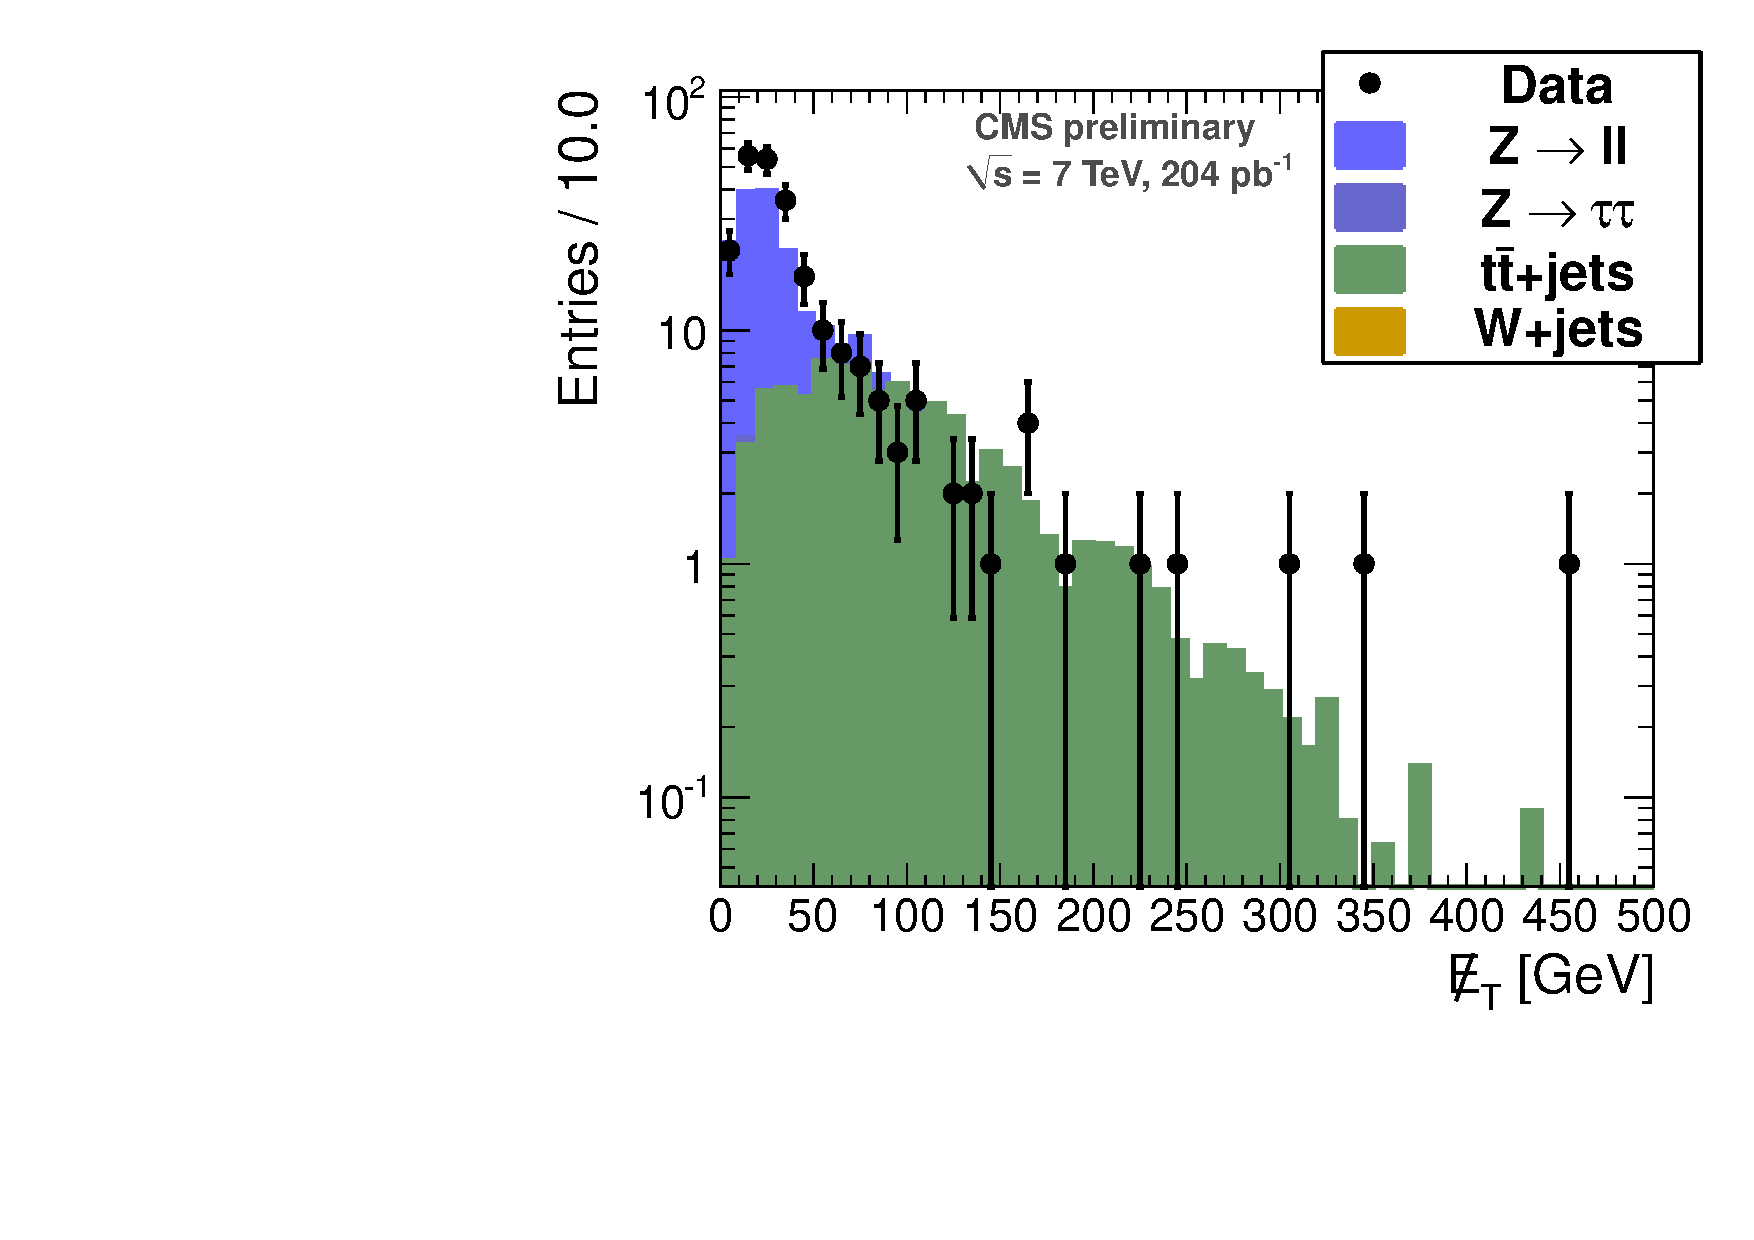
\includegraphics[width=0.79\textwidth]{Summer11_07_MC_pfLeptSusyCuts_Data_MET_2010.pdf}}\hfill
  \caption{\MET distribution for all events passing di-lepton selection and satisy $\HT> 350$~GeV. For the final \MET selection (150)~GeV the selection is dominated by $t\bar{t}$.}
\end{figure}

The \MET distribution after application of the \HT
cut is shown in Fig~\ref{fig:MET2010} and
the yield split by flavour for a cut at 150~GeV is listed in Tab.~\ref{tab:2010}.

\begin{table}[htb]
\begin{center}
\caption{\label{tab:2010}\protect Summary of number of events expected from Monte Carlo simulations in 
the signal region of $H_T> 350$~GeV and $\MET> 150$~GeV. The errors reflect the Monte Carlo (scaled
    to 204~\pbi) statistics only.}
\begin{tabular}{l|ccc|c}
\hline
Process           & $ee$       & $\mu\mu$     & $e\mu$   & total   \\
\hline\hline
$W+\textrm{jets}$&$0.0 \pm 0.0$&$0.0 \pm 0.0$&$0.0 \pm 0.0$&$0.0 \pm 0.0$\\
$Z\rightarrow ll+\textrm{jets}$&$0.0 \pm 1.97$&$0.0 \pm 1.97$&$0.0 \pm 1.97$&$0.0 \pm 0.27$\\
$Z \rightarrow \tau\tau$&$0.0 \pm 1.0$&$0.0 \pm 1.0$&$0.0 \pm 1.0$&$0.0 \pm 0.27$\\
$t\bar{t}$&$3.44 \pm 0.42$&$4.26 \pm 0.47$&$7.46 \pm 0.63$&$15.17 \pm 0.9$\\
\hline
Total background&$3.44 \pm 2.25$&$4.26 \pm 2.26$&$7.46 \pm 2.3$&$15.17 \pm 0.98$\\
\hline
Data  & 3 & 3 & 4 & 10 \\
\hline\hline
%LM0               &$3.41 \pm 0.17$&$3.91 \pm 0.17$&$4.52 \pm 0.14$&$11.84 \pm 0.42$ \\
%LM1               &$1.64 \pm 0.04$&$2.02 \pm 0.04$&$1.01 \pm 0.03$&$4.64 \pm 0.07$ \\
%\hline
\end{tabular}
\end{center}
\end{table}

\subsubsection{High \HT signal region}

A signal region with high \HT is defined by tightening the $\HT$ 
from the preselection region
\begin{itemize}
\item A $\HT>600$~GeV.
\item A $\MET>100$~GeV.
\end{itemize}

\begin{figure}[hbtp]
  \subfigure[]{\label{fig:METHighHT}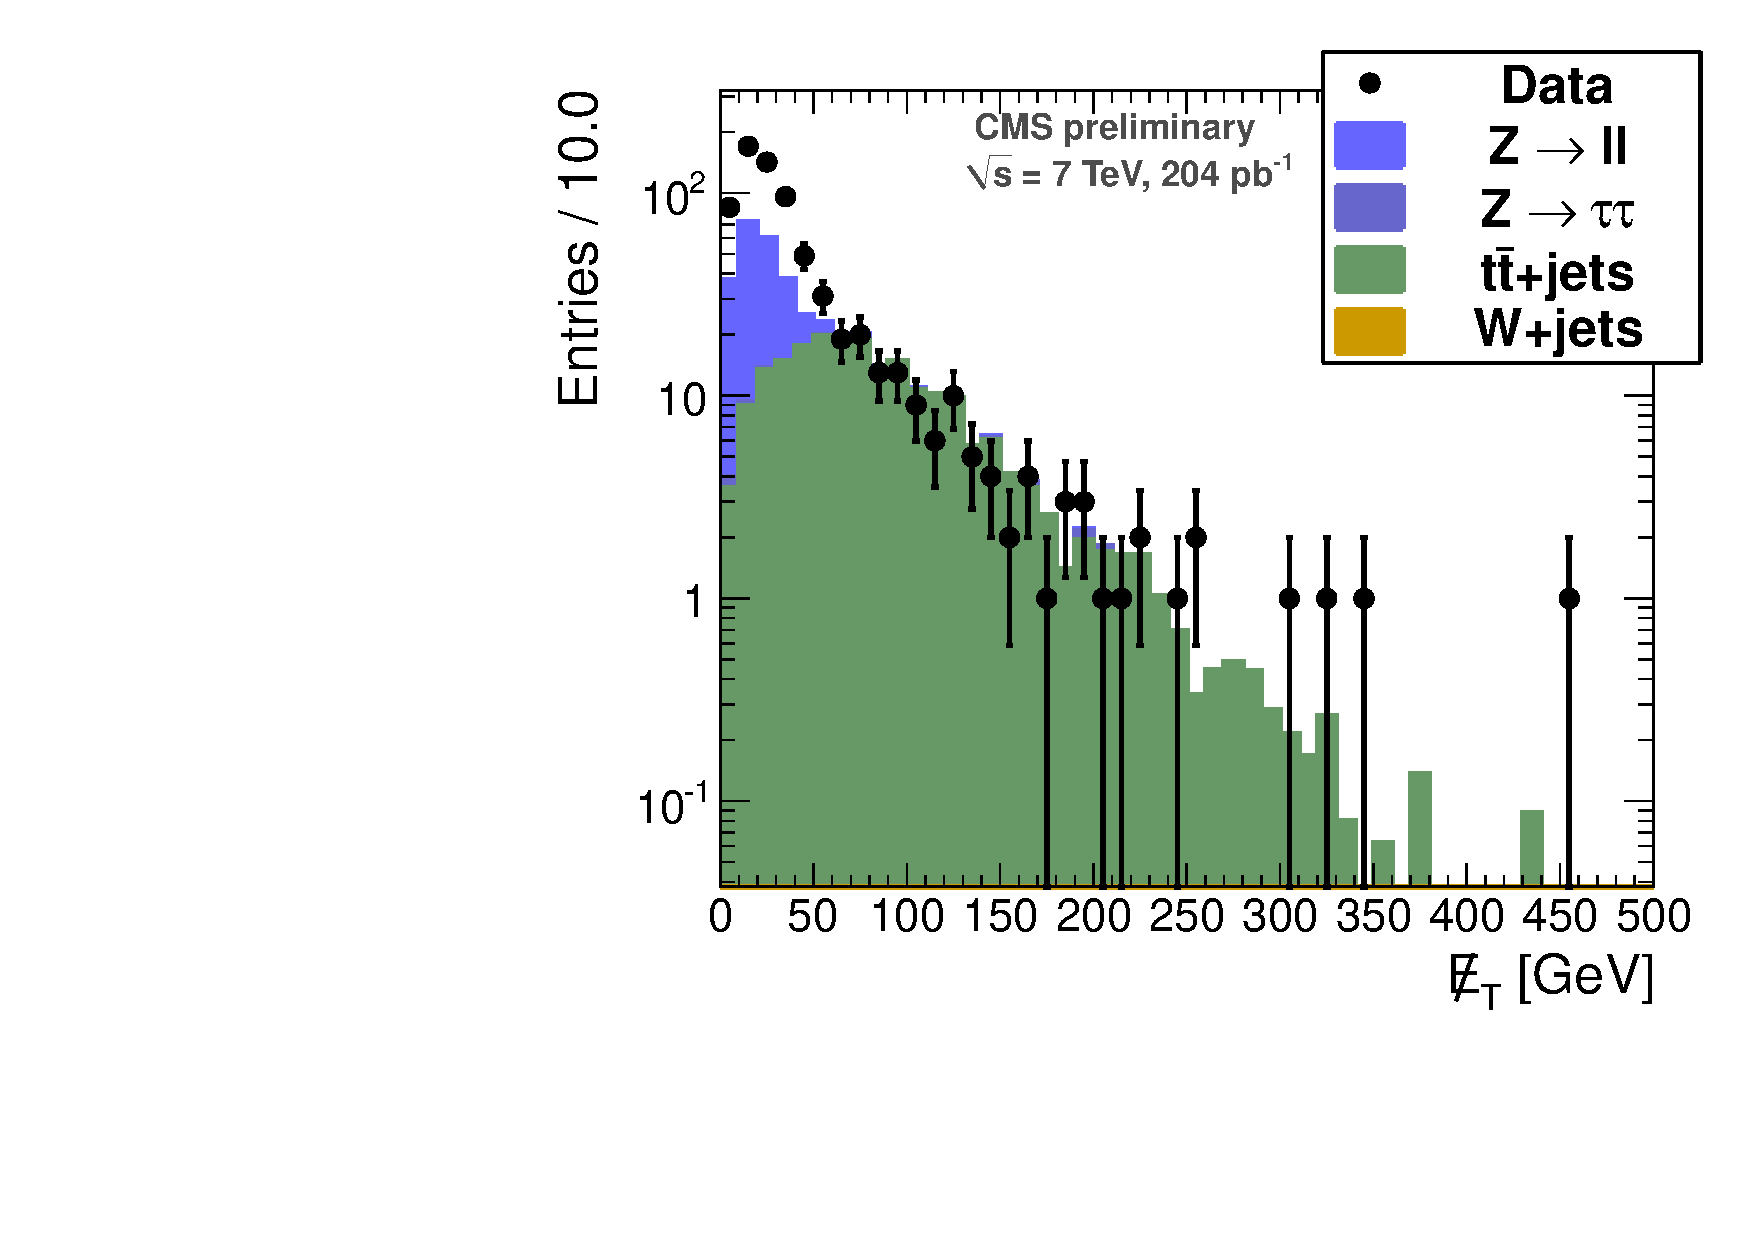
\includegraphics[width=0.79\textwidth]{Summer11_07_MC_pfLeptSusyCuts_Data_MET_HighMET.pdf}}\hfill
  \caption{\MET distribution for all events passing di-lepton selection and satisfy $\HT> 600$~GeV. For the final \MET selection (100)~GeV the selection is dominated by $t\bar{t}$.}
\end{figure}

The \MET distribution after application of the \HT
cut is shown in Fig~\ref{fig:METHighHT} and
the yield split by flavour for a cut at 150~GeV is listed in Tab.~\ref{tab:HighHT}.

\begin{table}[htb]
\begin{center}
\caption{\label{tab:HighHT}\protect Summary of number of events expected from Monte Carlo simulations in 
the signal region of $H_T> 600$~GeV and $\MET> 100$~GeV. The errors reflect the Monte Carlo (scaled
    to 204~\pbi) statistics only.}
\begin{tabular}{l|ccc|c}
\hline
Process           & $ee$       & $\mu\mu$     & $e\mu$   & total   \\
\hline\hline
$W+\textrm{jets}$&$0.0 \pm 0.0$&$0.0 \pm 0.0$&$0.0 \pm 0.0$&$0.0 \pm 0.0$\\
$Z\rightarrow ll+\textrm{jets}$&$0.08 \pm 1.47$&$0.0 \pm 1.97$&$0.0 \pm 1.97$&$0.08 \pm 3.15$\\
$Z \rightarrow \tau\tau$&$0.0 \pm 1.0$&$0.0 \pm 1.0$&$0.0 \pm 1.0$&$0.0 \pm 0.27$\\
$t\bar{t}$&$1.11 \pm 0.23$&$1.69 \pm 0.31$&$2.7 \pm 0.41$&$5.5 \pm 0.56$\\
\hline
Total background &$1.19 \pm 1.8$&$1.69 \pm 2.23$&$2.7 \pm 2.25$&$5.58 \pm 3.22$\\
\hline
Data  & 2 & 0 & 2 & 4 \\
\hline\hline
%LM0               &$3.41 \pm 0.17$&$3.91 \pm 0.17$&$4.52 \pm 0.14$&$11.84 \pm 0.42$ \\
%LM1               &$1.64 \pm 0.04$&$2.02 \pm 0.04$&$1.01 \pm 0.03$&$4.64 \pm 0.07$ \\
%\hline
\end{tabular}
\end{center}
\end{table}


\subsubsection{High \MET signal region}

A signal region with high \MET is defined by slightly tightening the $\HT$ 
and a much tighter $\MET$ selection compared to the pre-selection region
\begin{itemize}
\item A $\HT>250$~GeV.
\item A $\MET>250$~GeV.
\end{itemize}

\begin{figure}[hbtp]
  \subfigure[]{\label{fig:METHighHT}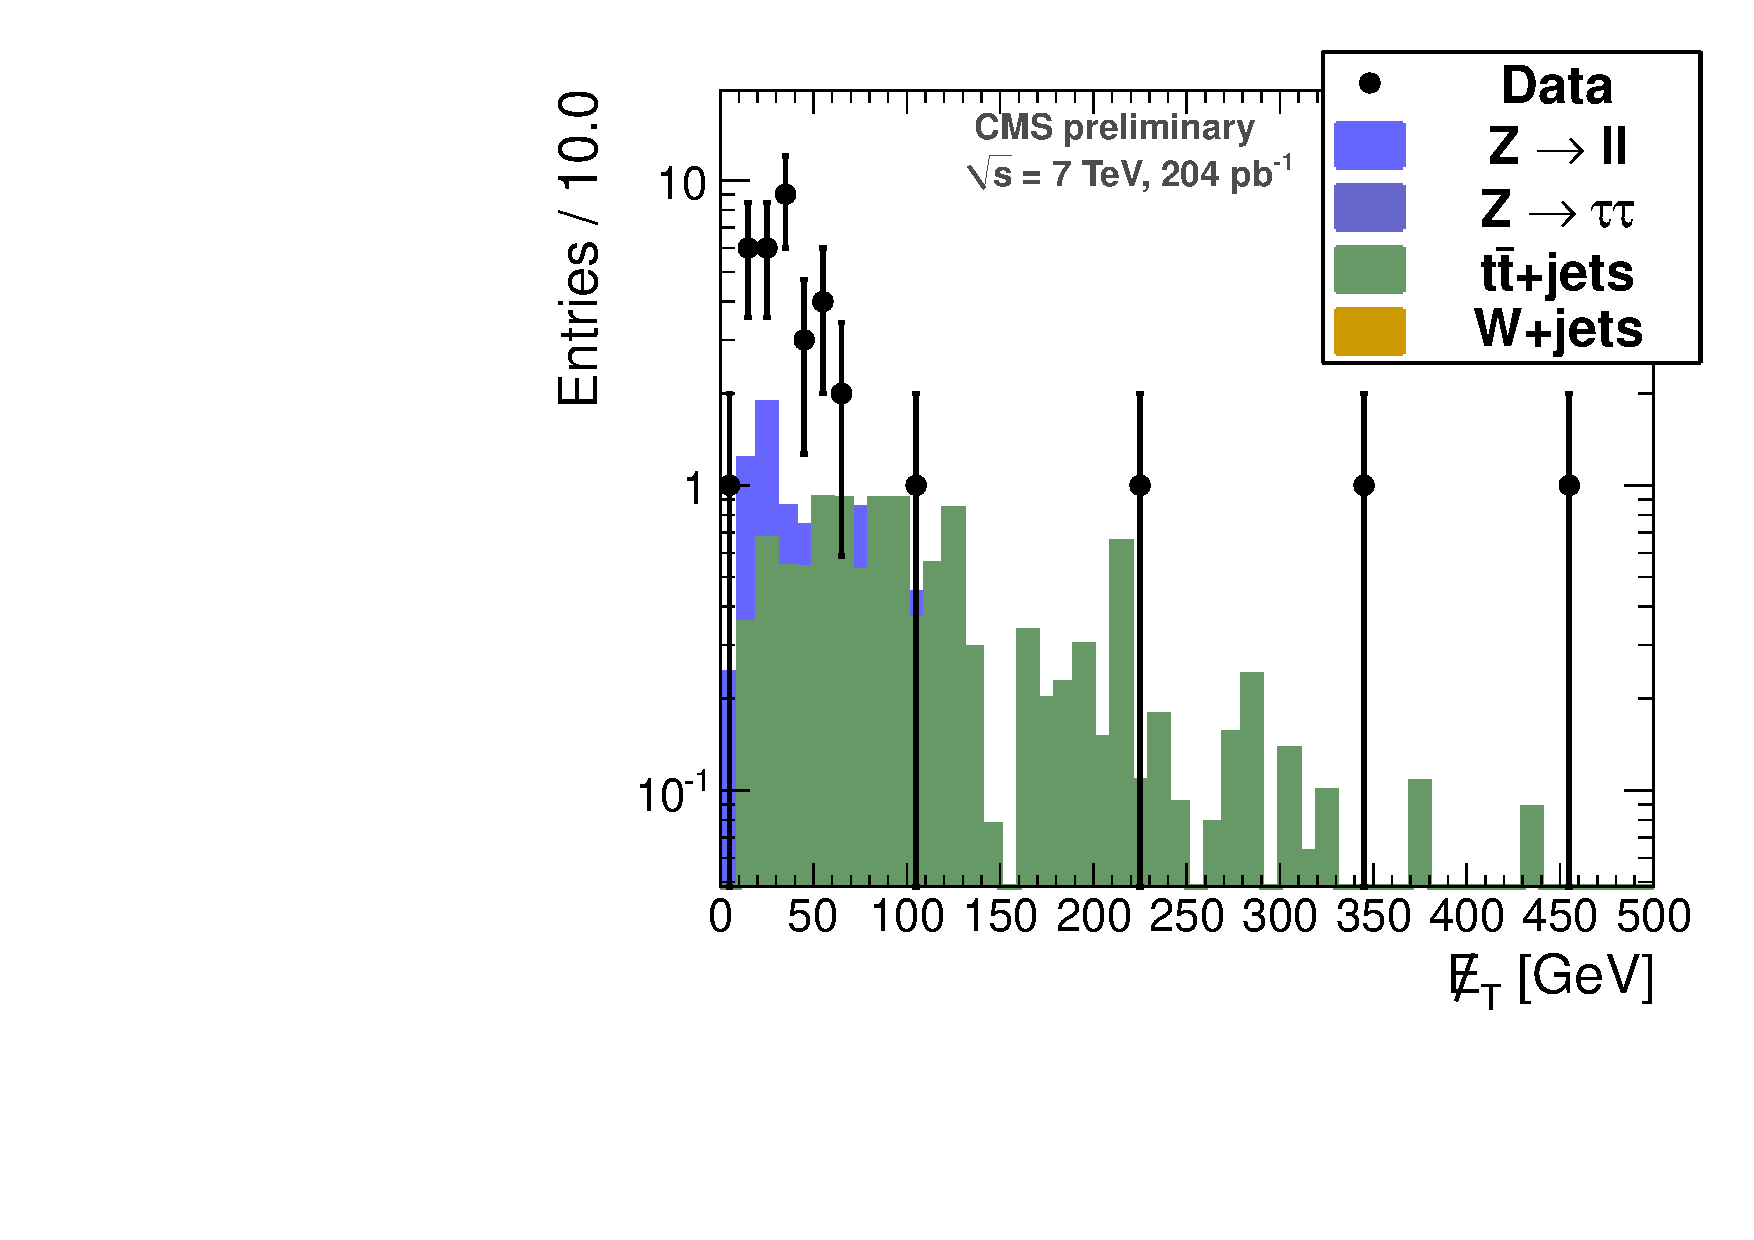
\includegraphics[width=0.79\textwidth]{Summer11_07_MC_pfLeptSusyCuts_Data_MET_HighHT.pdf}}\hfill
  \caption{\MET distribution for all events passing di-lepton selection and satisfy $\HT> 250$~GeV. For the final \MET selection (250)~GeV the selection is dominated by $t\bar{t}$.}
\end{figure}

The \MET distribution after application of the \HT
cut is shown in Fig~\ref{fig:METHighHT} and
the yield split by flavour for a cut at 250~GeV is listed in Tab.~\ref{tab:HighMET}.

\begin{table}[htb]
\begin{center}
\caption{\label{tab:HighMET}\protect Summary of number of events expected from Monte Carlo simulations in 
the signal region of $H_T> 250$~GeV and $\MET> 250$~GeV. The errors reflect the Monte Carlo (scaled
    to 204~\pbi) statistics only.}
\begin{tabular}{l|ccc|c}
\hline
Process           & $ee$       & $\mu\mu$     & $e\mu$   & total   \\
\hline\hline
$W+\textrm{jets}$ &$0.0 \pm 0.0$&$0.0 \pm 0.0$&$0.0 \pm 0.0$&$0.0 \pm 0.0$\\
$Z\rightarrow ll+\textrm{jets}$&$0.0 \pm 1.97$&$0.0 \pm 1.97$&$0.0 \pm 1.97$&$0.0 \pm 0.27$\\
$Z \rightarrow \tau\tau$&$0.0 \pm 1.0$&$0.0 \pm 1.0$&$0.0 \pm 1.0$&$0.0 \pm 0.27$\\
$t\bar{t}$&$0.4 \pm 0.16$&$1.0 \pm 0.23$&$1.68 \pm 0.28$&$3.08 \pm 0.4$\\
\hline
Total background &$0.4 \pm 2.22$&$1.0 \pm 2.22$&$1.68 \pm 2.23$&$3.08 \pm 0.56$\\
\hline
Data  & 3 & 0 & 3 & 6 \\
\hline\hline
%LM0               &$3.41 \pm 0.17$&$3.91 \pm 0.17$&$4.52 \pm 0.14$&$11.84 \pm 0.42$ \\
%LM1               &$1.64 \pm 0.04$&$2.02 \pm 0.04$&$1.01 \pm 0.03$&$4.64 \pm 0.07$ \\
%\hline
\end{tabular}
\end{center}
\end{table}

%\input{xsection}
\section{Background prediction methos}

\subsection{Different flavour subtraction} \label{sec:ofossubtraction}
Since the signal region is expected to be absolutely 
dominated by $t\bar{t}$-production we use
the opposite flavour subtraction to predict
backgrounds where uncorrelated leptons are being produced.
It relies only on the knowledge of the ratio
of electron to muon reconstruction efficiency $r_{e\mu}$,
which we derive in Sec.~\ref{sec:eff}.

Under the assumption of lepton unversality
The following two formulas hold for any background
where di-leptons are being produced uncorrelated 
(e.g. top-pairs events, $Z \rightarrow \tau^{+} \tau{-} \rightarrow 
l^{+} \l^-$, $WW$-production):
$$
n_{ee} = \frac12n_{e\mu}r_{\mu{}e}, \quad n_{\mu\mu} = \frac12\frac{n_{e\mu}}{r_{\mu{}e}}.
$$
A closure test of the method has been performed
using a simulated top-pair sample and
we observe a good agreement between prediction and MC truth:
$$
n_{ee} = 16.9 \pm 2.8 (\textnormal{stat.}) \; \textnormal{ (16.2 MC)}, \quad n_{\mu\mu} = 19.8 \pm 3.3 (\textnormal{stat.}) \; \textnormal{ (21.5 MC)}.
$$


\subsection{Control Region}

To gain confidence in the performance of this technique we wish to test it on a high statistic sample, dominated by 
$t\bar{t}$, as is our expected signal region is. To do this, we are required to use the leptonic trigger sample, 
described in~\cite{avi} including the lepton $p_T$ thresholds of 20 (10)~GeV, 
since we need to lower the $H_T$ requirement inherent in the hadronic trigger sample. Using 
this sample our control region is defined by:  $100 < H_T < 350$~GeV and $\MET>80$~GeV,
where we expect almost no Z+Jets contribution anymore and are dominated by $t\bar{t}$.
The control region is disjunct from the signal region, however it also suffers,
from potential signal contamination, in case of a very soft \MET spectrum of the new physics.
The distribution of the events in the invariant mass distribution split by lepton flavour combinations
is shown in Fig.~\ref{fig:control_InvMass}.

In this region we observe $26$ opposite flavour opposite sign candidates and
subtract $1.0\pm0.5$ predicted fake events. Therefore we obtain $25.0\pm0.5$ $t\bar{t}$-
like candidate events, which we use to obtain a prediction for the same flavour combinations
using the ratio of Tab.~\label{tab:tnp_eff}.

Table~\ref{tab:OFexpect} shows the number of expected SM background events in the control region $100 < H_T < 350$~GeV 
and $\MET>80$~GeV, as well as the prediction from the background estimation techniques, for an integrated
luminosity of 35~pb${}^{-1}$. We observe a good agreement between prediction and observation.

\begin{table}[hbt]
\begin{center}
\caption{\label{tab:OFexpect}Number of predicted and observed events in the control region, defined as: $100 < H_T < 350$~GeV and $\met > 80$~GeV.}
\begin{tabular}{l|cc}
\hline
                       & \multicolumn{2}{c}{Control Region}               \\
\hline 
Process                & $ee$          & $\mu\mu$        \\
\hline
$t\bar{t}$ from $e\mu$ & $11.7\pm 2.4$ & $13.4\pm 2.8$   \\
Fake leptons           & $0.5\pm 0.3$  & $0.4\pm0.2$                  \\
\hline
Total predicted        & $12.2\pm 2.4$ & $13.8 \pm 2.8$  \\
\hline\hline
Total observed         & $10$          & $15$          \\
\hline \hline
SM MC         & $8.4\pm 0.2$  & $10.5 \pm 0.3$    \\
LM0                    &  $3.7\pm0.2$  & $4.2\pm0.2$     \\
LM1                    &  $0.5\pm0.1$  & $0.7\pm0.1$     \\

\hline
\end{tabular}
\end{center}
\end{table}



%\input{jzbalance}
\section{Results}\label{sec:results}

In Tab.~\ref{tab:predict2010} the yields and the background predictions
from the three methods are listed for the signal region used for the analysis
of the 2010 data. Good agreement between prediction and
observation is seen.

\begin{table}[hbt]
\begin{center}
\caption{\label{tab:predict2010}Number of predicted and observed events in the 2010 signal region, 
    defined as: $H_T > 350$~GeV and $\met > 150$~GeV.}
\begin{tabular}{l|cc}
\hline
                       & \multicolumn{2}{c}{2010 signal region}               \\
\hline 
Process                & $ee$          & $\mu\mu$        \\
\hline
$t\bar{t}$ from $e\mu$ & $11.7\pm 2.4$ & $13.4\pm 2.8$   \\
Fake leptons           & $0.5\pm 0.3$  & $0.4\pm0.2$                  \\
\hline
Total predicted        & $12.2\pm 2.4$ & $13.8 \pm 2.8$  \\
\hline\hline
Total observed         & $10$          & $15$          \\
\hline \hline
SM MC         & $8.4\pm 0.2$  & $10.5 \pm 0.3$    \\
LM0                    &  $3.7\pm0.2$  & $4.2\pm0.2$     \\
LM1                    &  $0.5\pm0.1$  & $0.7\pm0.1$     \\

\hline
\end{tabular}
\end{center}
\end{table}


In Tab.~\ref{tab:predictHighMET} the yields and the background predictions
from the three methods are listed for the signal region defined by a tight
\MET selection. We observe good agreement between prediction
and observation.

\begin{table}[hbt]
\begin{center}
\caption{\label{tab:predictHighMET}Number of predicted and observed events in the high \MET signal region, 
    defined as: $H_T > 250$~GeV and $\met > 250$~GeV.}
\begin{tabular}{l|cc}
\hline
                       & \multicolumn{2}{c}{High \MET Region}               \\
\hline 
Process                & $ee$          & $\mu\mu$        \\
\hline
$t\bar{t}$ from $e\mu$ & $11.7\pm 2.4$ & $13.4\pm 2.8$   \\
Fake leptons           & $0.5\pm 0.3$  & $0.4\pm0.2$                  \\
\hline
Total predicted        & $12.2\pm 2.4$ & $13.8 \pm 2.8$  \\
\hline\hline
Total observed         & $10$          & $15$          \\
\hline \hline
SM MC         & $8.4\pm 0.2$  & $10.5 \pm 0.3$    \\
LM0                    &  $3.7\pm0.2$  & $4.2\pm0.2$     \\
LM1                    &  $0.5\pm0.1$  & $0.7\pm0.1$     \\

\hline
\end{tabular}
\end{center}
\end{table}

Tab.~\ref{tab:predictHighMET} compares the yields and the background predictions
from the three background prediction methods for the signal region defined by a tight
\HT selection. A good agreement between prediction and observation can be seen.

\begin{table}[hbt]
\begin{center}
\caption{\label{tab:predictHighMET}Number of predicted and observed events in the high \HT signal region, 
    defined as: $H_T > 600$~GeV and $\met > 100$~GeV.}
\begin{tabular}{l|cc}
\hline
                       & \multicolumn{2}{c}{High \HT region}               \\
\hline 
Process                & $ee$          & $\mu\mu$        \\
\hline
$t\bar{t}$ from $e\mu$ & $11.7\pm 2.4$ & $13.4\pm 2.8$   \\
Fake leptons           & $0.5\pm 0.3$  & $0.4\pm0.2$                  \\
\hline
Total predicted        & $12.2\pm 2.4$ & $13.8 \pm 2.8$  \\
\hline\hline
Total observed         & $10$          & $15$          \\
\hline \hline
SM MC         & $8.4\pm 0.2$  & $10.5 \pm 0.3$    \\
LM0                    &  $3.7\pm0.2$  & $4.2\pm0.2$     \\
LM1                    &  $0.5\pm0.1$  & $0.7\pm0.1$     \\

\hline
\end{tabular}
\end{center}
\end{table}


We find one event in the signal region in the $e\mu$-lepton combination with a fake prediction
of $0.1\pm0.1$, and thus predict $0.9 {}_{-0.8}^{+2.2}$ same-flavour events.
In data we find no same-flavour events and have to contrast this with $7.3\pm1.6$ and ($3.6\pm0.7$) expected
events at the benchmark points LM0 (LM1).




\section{Systematic uncertainties}\label{sec:systematics}

Systematic uncerteinties arise from uncertainties of the event selection
expected in simulation compared to the performance from the actual detector.
A global normalisation uncertainty comes from an uncertainty on the total 
integrated luminosity of 11\%~\cite{lumiCMS}.

\subsection{Systematic uncertainty for the lepton selection}

We do observe a good agreement from tag and probe within 2\%.
In simulation the difference of the lepton
selection between Z+jets and top-pair events is within 7\%,
which we use as a systematic uncertainty.
The inclusive lepton efficiency of leptons in the mSUGRA
benchmark points differ by 25\% to the efficiency measured
at the Z resonace. 
However this drop in efficiency is simulated by the MC.
We take 10\% uncertainty on the leptonic part as a systematic uncertainty in the
limit setting procedure.

\subsection{Pile-up}

Since the lepton efficiency is measured including pile-up, we  include the effect
and do not correct for the difference in lepton selection efficiency.
Nevertheless pile-up has some effect on the jet and missing transvers energy 
selection. It has been studied in simulation and found to be negligible for the high \HT
and \MET selection.
Therefore no additional uncertainty is assigned to account for
pile-up.
For leptons above 10~GeV the effect of pile-up in the isolation is below 3\%
per lepton and therefore we do not assign an additional systematic uncertainty.

\subsection{Uncertainty on the hadronic selection}

The uncertainty on the jet-energy-scale is smaller than 5\% for
particle flow jets~\cite{jetMETUncertainty}. This uncertainty
directly translates into a scale uncertainty on the \HT selection.
For particle flow MET and uncertainty on the scale of 5\% is assumed~\cite{pfMETUNcertainty}.
We vary both fully correlated and find that it changes the acceptance
at LM0 by 12\%, while the change at LM1 is smaller (5\%).
We take this as systematic uncertainty in the limit setting method.
The uncertainty in the $t\bar{t}$-sample is found to be 30\%
in the final signal selection, while it is smaller in the leptonic control region (7\%). 
This enters the predicted number from simulation.

\subsection{Uncertainty on the fake background prediction}

For the fake-component of the background a uncertainty of 50\% is assumed,
which is described in detail in Sec.~\ref{sec:fakes}.

The main uncertainty for the opposite flavour subtraction arises from
the uncertainty on the lepton selection in a hadronic event environment.
While the inclusive efficiency for leptons originating from the Z-Boson
can be determined with a systematic uncertainty of 2\%, it cannot be 
determined with that precision in the kinematic regime of the search.
Therefore the difference between the efficiency from the Z and $t\bar{t}$
is assumed as a systematic uncertainty (5\%).

The systematic uncertainties on the yields from simulation are
summarised in Tab.~\ref{tab:systematics}.

\begin{table}[hbtp]
\caption{Summary of the systematic uncertainties for \label{tab:systematics}}
\begin{center}
\begin{tabular}{|l||c|c|c|} \hline
Systematic uncertainty    &   $t\bar{t}$   &   LM0        & LM1\\\hline \hline
Cross-section &   39\% & -    &- \\\hline  
\HT + \MET &   30\% & 12\%    &5\% \\\hline  
Lepton &   10\% & 15\%    &15\% \\\hline  
Luminosity &   11\% & 11\%    &11\% \\\hline\hline
Total &   51\% & 22\%    &19\% \\\hline  
\end{tabular}
\end{center}
\end{table}


\section{Limit}\label{sec:significance}

As discussed in Section~\ref{sec:results}, we see no event 
in the signal region, defined as $H_T>$350~GeV and 
$\MET>150$~GeV and two same flavour opposite sign leptons.

The background prediction from the SM Monte Carlo is 
0.77 $\pm$ 0.26 events, where the uncertainty comes from 
the jet energy scale (30\%, see Section~\ref{sec:systematics}),
the luminosity (11\%), and the lepton/trigger 
efficiency (10\%)\footnote{Other uncertainties associated with 
the modeling of $t\bar{t}$ in MadGraph have not been evaluated.}.
The opposite flavor based background prediction is $0.9 {}_{-0.8}^{+ 2.2}$.

The background prediction is well in agreement with the prediction from
simulation and with the observation of no events.

We calculate a Bayesian 95\% CL upper limit~\cite{bayes} 
on the number of non SM events in this signal region to be 3.0.

We cross-checked the code with a Bayesian 95\% CL upper limit using the MCMC calculator\cite{roostats} 
and get the same result of 3.0.

Here as well, we remind the reader of the number of expected
LM0 and LM1 events from Table~\ref{tab:expect}: $7.3 \pm 1.6$ 
events and $3.3 \pm 0.7$ respectively, where the uncertainties
are from energy scale (Section~\ref{sec:systematics}), luminosity,
and lepton efficiency.

We thus can exclude LM0 95\% confidence level.

\section{Conclusion}

%We have presented a SUSY search for correlated flavour production in the opposite-sign channel
%in the presence of high \HT and \MET.
%We observe good agreement between data and simulation as well as to our background prediction
%method.
%We conclude that there is no sign of flavour correlated production and set a limit $3.0$
%signal events at 95\% confidence level within acceptance of our selection. 
%This excludes the discussed benchmark points LM0.

%============



\section{Acknowledgements}

\begin{thebibliography}{9}
    \bibitem{softsusy} B.C.~Alanach, {\em "SOFTSUSY: a program for calculating supersymmetric spectra"}, Comput.Phys.Commun. 143:305-331, 2002
    
    \bibitem{susyhit} A.~Djouadi et al, {\em Decays of Supersymmetric Particles: the program SUSY-HIT (SUspect-SdecaY-Hdecay-InTerface)} ActaPhys.Polon. B38:635-644, 2007.

    \bibitem{pythia} T.~Sjostrand et al, {\em "PYTHIA 6.4 Physics and Manual"}, JHEP 0605:026, 2006

    \bibitem{prospino} W.~Beenakker et al, {\em "Squark and Gluino Production at Hadron Colliders"}, Nucl.Phys. B492:51-103, 1997
    
    \bibitem{zprod} The CMS Collaboration, {\em "Study of the Z production in association with jets in proton-proton collisions at $\sqrt{s}=10$~TeV with the CMS detector at the CERN LHC"}, CMS Physics Analysis Summary JME-08-006

    
    %\bibitem{alpgen} M.L.~Mangano et al, {\em "ALPGEN, a generator for hard multiparton processes in hadronic collisions"}, JHEP 0307:001, 2003

    \bibitem{antiKT} M.~Cacciar et al, {\em "The anti-$k_t$ jet clustering algorithm"}, JHEP 0804:063, 2008

    \bibitem{madgraph} J.~Alwall et al, {\em "MadGraph/MadEvent v4: The New Web Generation"}, JHEP 0709:028, 2007
    
    \bibitem{ttkfactor} M.~Cacciari et al, {\em "Updated predictions for the total production cross sections of top and of heavier quark pairs at the Tevatron and at the LHC"}, JHEP 0809:127, 2008
    
    \bibitem{WZkfactor} S.~Frixione, M.L.~Mangano, {\em "How accurately can we measure the W cross section?"}, JHEP 0405:056, 2004
    
    \bibitem{sPlot} M.~Pivk and F.R.~Le~Diberder, {\em A statistical tool to unfold data distributions}, arXiv:physics/0402083    

    \bibitem{vplus} V+jets wiki, \url{https://twiki.cern.ch/twiki/bin/view/CMS/VplusJets}

    \bibitem{muons} M.~Mulders et al. {\em "Muon Identification in CMS"}, CMS Analysis Note 2008/098
    
    \bibitem{electrons} J.~Branson et al. {\em "A cut based method for electron identification in CMS"}, CMS Analysis Note 2008/082

    \bibitem{pfelectrons} F.~Beaudette et al. {\em "Electron Reconstruction within the Particle Flow Algorithm"}, CMS Analysis Note 2010/034
    \bibitem{particleflow} M.~Bachtis et al. {\em "Commissioning of
        the Particle-flow Event Reconstruction with the first LHC
        collisions recorded in the CMS detector"}, CMS Analysis Note 2010/???
     
    \bibitem{SIScone} G.~P.~Salam, G.~Soyez, {\em "A practical Seedless Infrared-Safe Cone jet algorithm"}, JHEP 0705:086, 2007 
    
    \bibitem{mcjetcorrections} The CMS Collaboration, {\em "Plans for Jet Energy Corrections at CMS"}, CMS Physics Analysis Summary JME-07-002
   
    \bibitem{pfjetid}N. Saoulidou, {\em "Particle Flow Jet
        Identification Criteria"}, CMS Analysis Note 2009/???

    \bibitem{roofit} W.~Verkerke, D.~Kirkby, {\em "The RooFit toolkit for data modeling"}, arXiv:physics/0306116
    
    \bibitem{muonPerformance} The CMS Collaboration, {\em "Performance of muon identification in pp collisions at $\sqrt{s}= 7$~TeV"}, CMS Physics Analysis Summary MUO-10-002

    \bibitem{suspas10001} The CMS Collaboration, {\em "Performance of Methods for Data-Driven Background Estimation in SUSY Searches"}, CMS Physics Analysis Summary SUS-10-001
    
    \bibitem{kostas} K.~Theofilatos et al. {\em "SUSY Searches in the $Z^0+3$ jets + \MET Final State with Data-driven Background Estimation"}, CMS Analysis Note 2009/132
    
    \bibitem{anil}  A.~Singh et al. {\em "SUSY in the $Z/\gamma*+$ Jet(s) + \MET Final State Using Particle Flow"}, CMS Analysis Note 2010/250
    
    \bibitem{avi} B.~Hooberman et al. {\em "Search for new physics in the opposite sign dilepton sample"}, CMS Analysis Note 2010/370
    %\bibitem{METcorrections} The CMS Collaboration, {\em "$\not\!\!E_{T}$ performance in CMS"}, CMS Physics Analysis Summary JME-07-001

    %\bibitem{electronTnP} The CMS Collaboration, {\em "Measuring Electron Efficiencies at CMS with Early Data"}, CMS Physics Analysis Summary EGM-07-001
    
    
    %\bibitem{triggermenu} Lean Trigger Menu V0.3 wiki, \url{https://twiki.cern.ch/twiki/bin/view/CMS/TSG_18_II_09}
    
    %\bibitem{georgia} G.~Karapostoli et al., {\em "Dilepton + Jets + MET channel : Observation and Measurement of $\tilde{\chi}_2^0 \rightarrow \tilde{\chi}_1^0 ll$"}, CMS Note 2008/038


    \bibitem{pileup} J.~Conway, \url{https://twiki.cern.ch/twiki/bin/view/CMS/PileupInformation}
    \bibitem{bayes} J.~Conway, \url{http://www-cdf.fnal.gov/physics/statistics/code/bayes.f}
    \bibitem{roostats} RooStats wiki, \url{https://twiki.cern.ch/twiki/bin/view/RooStats/WebHome}

    %\bibitem{statistics} R.~D.~Cousins et al., {\em Evaluation of three methods for calculating statistical significance when incorporating a systematic uncertainty into a test of the background-only hypothesis for a Poisson process}, Nuclear Instruments and Methods in Physics Research A595:480-501, 2008
    
    \bibitem{lumiCMS} The CMS Collaboration, {\em "Measurement of CMS Luminosity"}, CMS Physics Analysis Summary EWK-10-004
    
    \bibitem{jetMETUncertainty} The CMS Collaboration, {\em "Jet Energy Corrections determination at $\sqrt{s}=7$~TeV"}, CMS Physics Analysis Summary JME-10-010
    
    \bibitem{pfMETUNcertainty} The CMS Collaboration, {\em "MET Performance in Events Containing Electroweak Bosons from pp Collisions at $\sqrt{s}=7$~TeV"}, CMS Physics Analysis Summary JME-10-005

\end{thebibliography}

\pagebreak
\appendix





\end{document}
